\section{问题一：感官评分的多输出回归与分级}

\subsection{问题描述}

问题一给出 \textbf{250} 个啤酒样本的 \textbf{231} 个化学特征，要求预测每个样本在 \textbf{50} 个感官维度上的评分，并把连续预测转成题面规定的 \textbf{0--6} 级整数。记化学特征矩阵为 $X\in\mathbb{R}^{250\times 231}$，感官标签矩阵为 $Y\in\mathbb{R}^{250\times 50}$，第 $d$ 个感官维度的标签为 $y_d$。学习目标是构造映射 $f_d\colon\mathbb{R}^{231}\to\mathbb{R}$，使折外预测 $\hat y_d=f_d(X)$ 与 $y_d$ 的误差尽可能小；随后用固定规则把 $\hat y_d$ 转成整数等级 $s_d\in\{0,1,\ldots,6\}$。

这一问的困难不在单个回归器的实现，而在三组矛盾。第一，特征多、样本少：\textbf{231} 个特征对应 \textbf{250} 个样本，若用线性模型，共线性会把系数估计放大；第二，多输出之间并不独立：麦芽香、酒花香、酯香等维度在感官上相关，逐维建模会重复利用同一批信息；第三，连续预测与离散评分之间存在“刻度差”：题面要的是 \textbf{0--6} 的等级，而模型输出的是条件均值，二者的分布形态并不相同。本文的模型设计分别回应这三组矛盾。

\subsection{模型建立}

\subsubsection{多输出随机森林}

本文把 \textbf{50} 个感官维度视为 \textbf{50} 个独立的回归任务，共用一个随机森林结构。随机森林由 $T$ 棵回归树组成，第 $t$ 棵树在自助采样得到的训练子集上生长，叶节点取该节点样本标签的均值。对输入 $x$，森林预测为
\begin{equation}
\hat y_d(x)=\frac{1}{T}\sum_{t=1}^{T}\hat y_{d,t}(x),
\label{eq:rf}
\end{equation}
其中 $\hat y_{d,t}(x)$ 是第 $t$ 棵树对第 $d$ 维的输出。树的每次分裂选择使左右子节点平方误差之和下降最多的特征与切分点，即
\begin{equation}
\Delta \mathrm{SSE}= \mathrm{SSE}(S)-\mathrm{SSE}(S_L)-\mathrm{SSE}(S_R),
\label{eq:split}
\end{equation}
其中 $S$ 为当前节点样本集，$S_L$、$S_R$ 为切分后的左右子集。随机森林在每次分裂时只随机考虑一部分特征，并对样本做有放回采样，因而能降低单棵树的方差，适合本题这种特征相关、样本有限的场景\cite{zhou2016,breiman2001}。

本文不把 \textbf{50} 个维度合并成一个多任务模型，而是逐维独立训练。这样做的好处是每一维的损失只由该维标签决定，不会因为某些维度量纲不同而互相牵制；代价是计算量随维度线性增加。考虑到 \textbf{50} 维、\textbf{250} 样本的规模，这一代价可以接受。

\subsubsection{ALR 分级标定}

连续预测 $\hat y_d$ 不能直接四舍五入成 \textbf{0--6}：不同维度的标签取值范围不同，直接取整会把大量样本压到 \textbf{0} 或 \textbf{1}。本文采用分维锚定线性映射加四舍五入（Anchor--Linear--Round，ALR）。对第 $d$ 维，取标签的 \textbf{0.5\%} 与 \textbf{99.5\%} 分位数为锚点 $lo_d$、$hi_d$，先做线性映射
\begin{equation}
s_d^{\ast}=6\cdot\frac{\hat y_d-lo_d}{hi_d-lo_d},
\label{eq:alr-linear}
\end{equation}
再按“半数向上”取整并截断：
\begin{equation}
s_d=\min\left\{6,\max\left\{0,\left\lfloor s_d^{\ast}+0.5\right\rfloor\right\}\right\}.
\label{eq:alr-round}
\end{equation}
式 \eqref{eq:alr-linear} 把不同量纲的预测拉到同一把 \textbf{0--6} 尺子上，式 \eqref{eq:alr-round} 保证输出是整数且不越界。锚点只从标签分布估计，不从预测分布估计；这一点是后文“刻度不可达命题”的前提，也是本文不通过拉伸预测去填补空等级的原因。

\subsubsection{评价指标}

连续预测用决定系数和平均绝对误差评价：
\begin{equation}
R^2=1-\frac{\sum_{i=1}^{n}(y_i-\hat y_i)^2}{\sum_{i=1}^{n}(y_i-\bar y)^2},\qquad
\mathrm{MAE}=\frac{1}{n}\sum_{i=1}^{n}\left|y_i-\hat y_i\right|.
\label{eq:metrics}
\end{equation}
$R^2$ 越接近 \textbf{1} 表示拟合越好，负值表示不如直接用均值预测；MAE 越小表示平均绝对偏差越小。分级结果另用单调性、保序性、等级覆盖、往返一致性和信息损失等指标检验，具体判据在第 \ref{sec:q1-check} 节给出。

\subsection{算法求解}

\subsubsection{预处理与验证设计}

预处理严格按第 \textbf{3} 章登记的口径执行：按 \texttt{beer} 键对齐 \textbf{250} 个样本；对 \textbf{33} 个原始量纲列做 \texttt{log10}$(x+10^{-6})$；在训练折内按风格分组取中位数插补 \textbf{73} 个缺失格，并保留 \textbf{9} 个缺失标记列；在训练折内做 z-score 标准化；\textbf{50} 维标签保持原值；全部 \textbf{250} 行参与建模。

交叉验证采用固定五折，每折 \textbf{50} 个样本，随机种子为 \textbf{2026}。所有模型、所有特征集、所有维度共用同一组折索引，折外预测由五折测试段拼接而成。这样得到的 OOF 预测既用于连续指标，也用于 ALR 分级；全量重训模型的样本内预测只用于推理接口自测，不进入任何论文数值。

随机森林的超参数在建模前冻结：树数 \textbf{500}，最大深度 \textbf{8}，叶节点最少样本 \textbf{3}，每次分裂随机考虑 \textbf{33\%} 的特征，随机种子 \textbf{2026}。本文不做网格搜索，也不逐维调参，避免在 \textbf{50} 维上产生选择偏差。

\subsubsection{两阶段模型选择}

模型选择分两阶段预注册，第二阶段只看一个指标。第一阶段固定 \textbf{230} 维特征集 F1，比较岭回归、随机森林和直方图梯度提升机；岭回归只作线性对照，不参与选型。第二阶段用胜出的随机森林分别跑 \textbf{226} 维的 F0、\textbf{230} 维的 F1 和 \textbf{231} 维的 F2，按“提升不足 \textbf{0.02} 就不加特征”的三步决策表判定。这个阈值在跑结果之前写入方案，结果出来之后不回改。

三步决策的逻辑是：若 F2 相对 F1 的提升达到 \textbf{0.02}，采用 F2；否则若 F1 相对 F0 的提升达到 \textbf{0.02}，采用 F1；否则采用最简的 F0。该规则把“特征更多是否真的有用”变成一个可复算的阈值判断，而不是凭测试集表现挑一套特征。

\subsubsection{求解流程}

求解按以下顺序执行：读取 \texttt{1.csv} 与 \texttt{4.csv} 并按 \texttt{beer} 对齐；按第 \textbf{3} 章的六步预处理生成训练折与测试折；在 F1 上训练三个候选模型并记录五折平均 $R^2$；用胜出的随机森林在 F0、F1、F2 上重复同一组折；按决策表选出主模型与主特征集；用五折 OOF 预测做 ALR 标定，得到 \textbf{250}$\times$\textbf{50} 的评分表；最后计算 T1--T8、E1--E3 与缺失鲁棒性指标。整条流程只依赖固定折索引与固定随机种子，冷跑与复跑应逐格一致。

\subsection{求解结果}

\subsubsection{模型与特征集}

模型选择结果如表 \ref{tab:q1-select} 所示。第一阶段中，随机森林的五折平均 $R^2$ 为 \textbf{0.2304}，明显高于直方图梯度提升机的 \textbf{0.1343}；岭回归为 \textbf{-0.6585}，说明线性模型在 \textbf{231} 维共线特征上严重过拟合。第二阶段中，F0、F1、F2 的平均 $R^2$ 分别为 \textbf{0.2305}、\textbf{0.2304}、\textbf{0.2317}，F1 相对 F0 的变化为 \textbf{-0.000095}，远小于 \textbf{0.02} 的阈值，因此决策表命中步骤 \textbf{3}，采用 F0。

\begin{table}[H]
\centering
\zihao{5}
\begin{tabularx}{\textwidth}{@{}p{0.10\textwidth}p{0.18\textwidth}rrrrX@{}}
\toprule
阶段 & 方案 & 特征数 & 折均 $R^2$ & OOF 全局 $R^2$ & 折均 MAE & 判定 \\
\midrule
阶段一 & 岭回归（对照） & \textbf{230} & \textbf{-0.6585} & \textbf{-0.4977} & \textbf{0.5039} & 不参与选型 \\
阶段一 & 随机森林 & \textbf{230} & \textbf{0.2304} & \textbf{0.2579} & \textbf{0.3390} & 主模型 \\
阶段一 & 直方图梯度提升机 & \textbf{230} & \textbf{0.1343} & \textbf{0.1850} & \textbf{0.3524} & 候选 \\
阶段二 & 随机森林 $\times$ F0 & \textbf{226} & \textbf{0.2305} & \textbf{0.2565} & \textbf{0.3394} & 采用 \\
阶段二 & 随机森林 $\times$ F1 & \textbf{230} & \textbf{0.2304} & \textbf{0.2579} & \textbf{0.3390} & 否 \\
阶段二 & 随机森林 $\times$ F2 & \textbf{231} & \textbf{0.2317} & \textbf{0.2583} & \textbf{0.3387} & 否 \\
\bottomrule
\end{tabularx}
\caption{问题一的模型选型与特征集决策}
\label{tab:q1-select}
\end{table}

表 \ref{tab:q1-select} 中“折均 $R^2$”是五个测试折上 \textbf{50} 维平均 $R^2$ 的再平均，“OOF 全局 $R^2$”是把五折测试段拼成 \textbf{250} 行后一次性计算的全局值，两者不可混比。主模型在 OOF 全局口径下为 \textbf{0.2565}，高于同口径的基线 \textbf{0.243}；在同折基线口径下，折均 \textbf{0.2305} 也高于 \textbf{0.2122}。两种口径下都不低于基线，说明增益不是换口径造成的。

\begin{figure}[H]
\centering
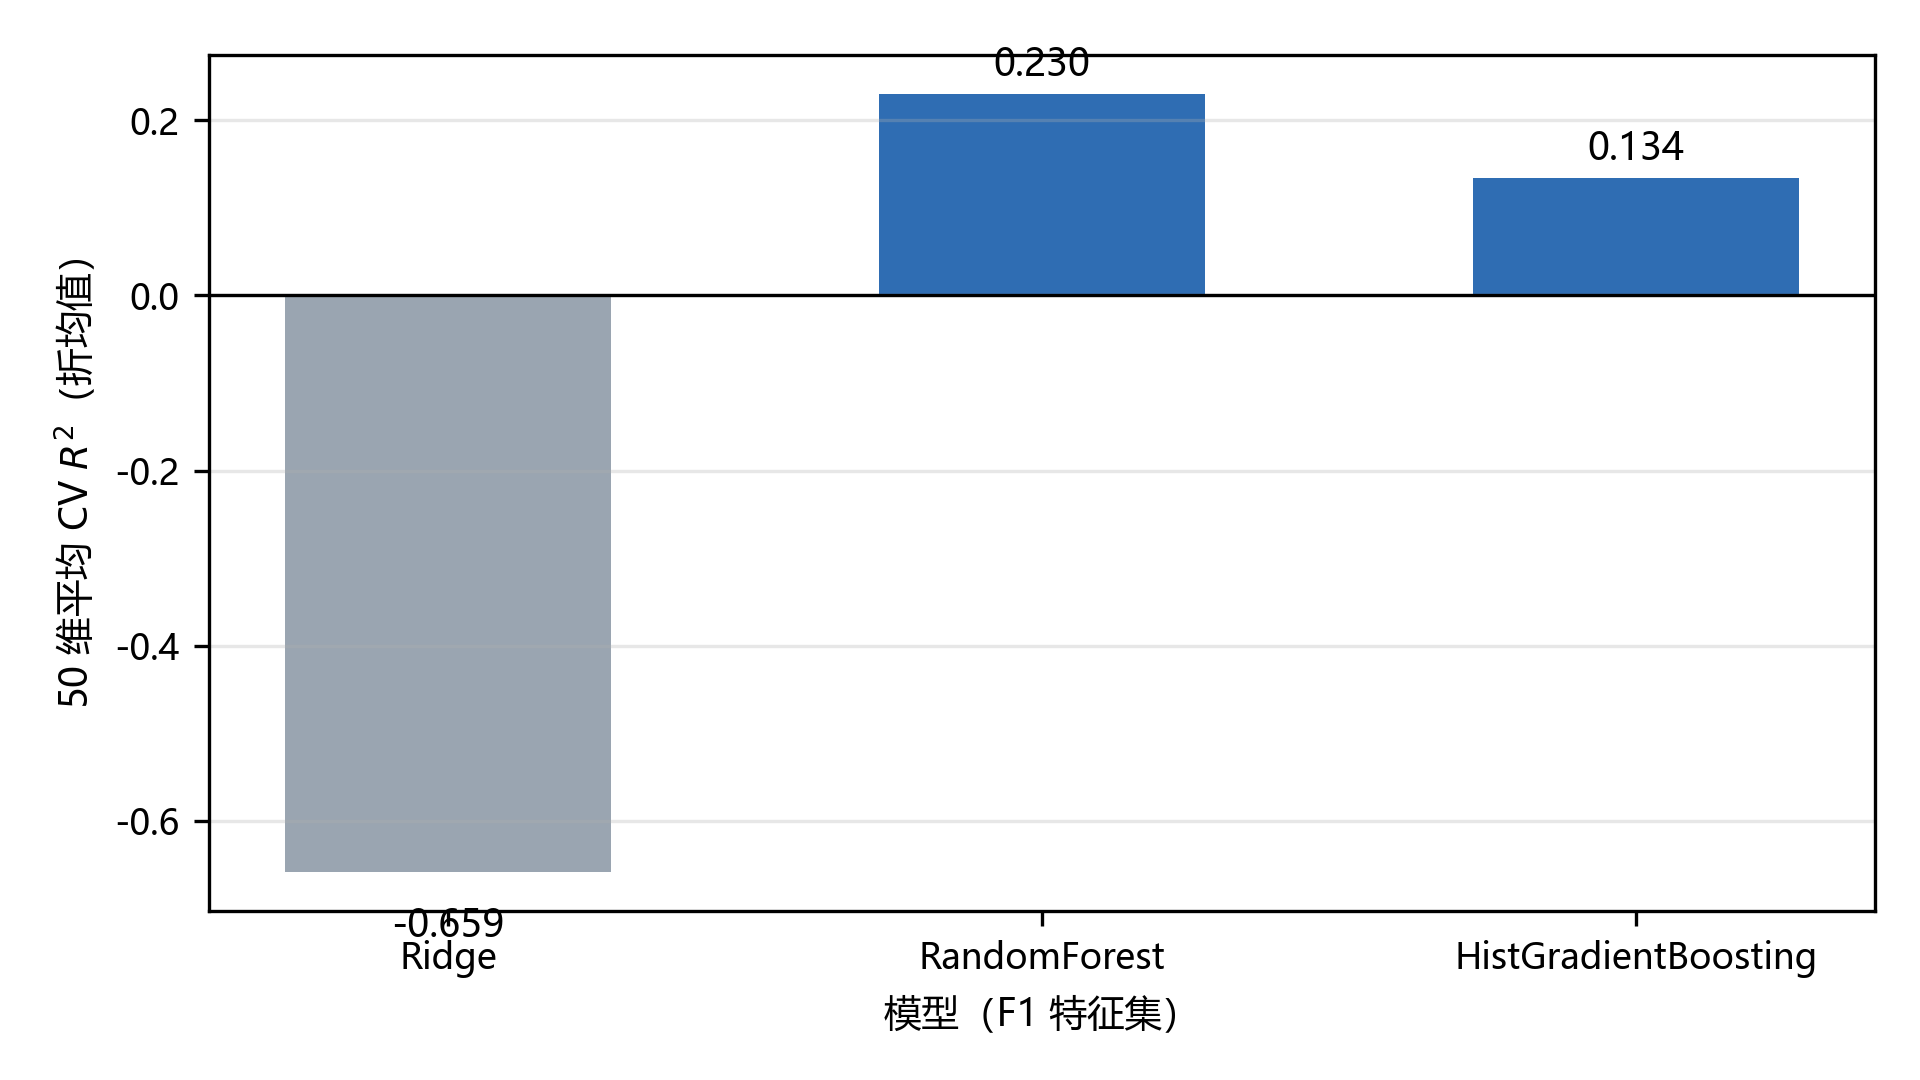
\includegraphics[width=0.68\textwidth]{图M3-01-模型选型对比.png}
\caption{三个候选模型在 F1 特征集上的 \textbf{50} 维平均交叉验证 $R^2$}
\label{fig:q1-model}
\end{figure}

图 \ref{fig:q1-model} 把三种模型的差距压缩成一张条形图：随机森林的柱高明显高于梯度提升机，岭回归则落到零线以下。需要说明的是，岭回归的负值不是“模型坏了”，而是线性假设与本题的强非线性、强共线性不匹配；它的作用只是提供一个“线性不可用”的对照。

\begin{figure}[H]
\centering
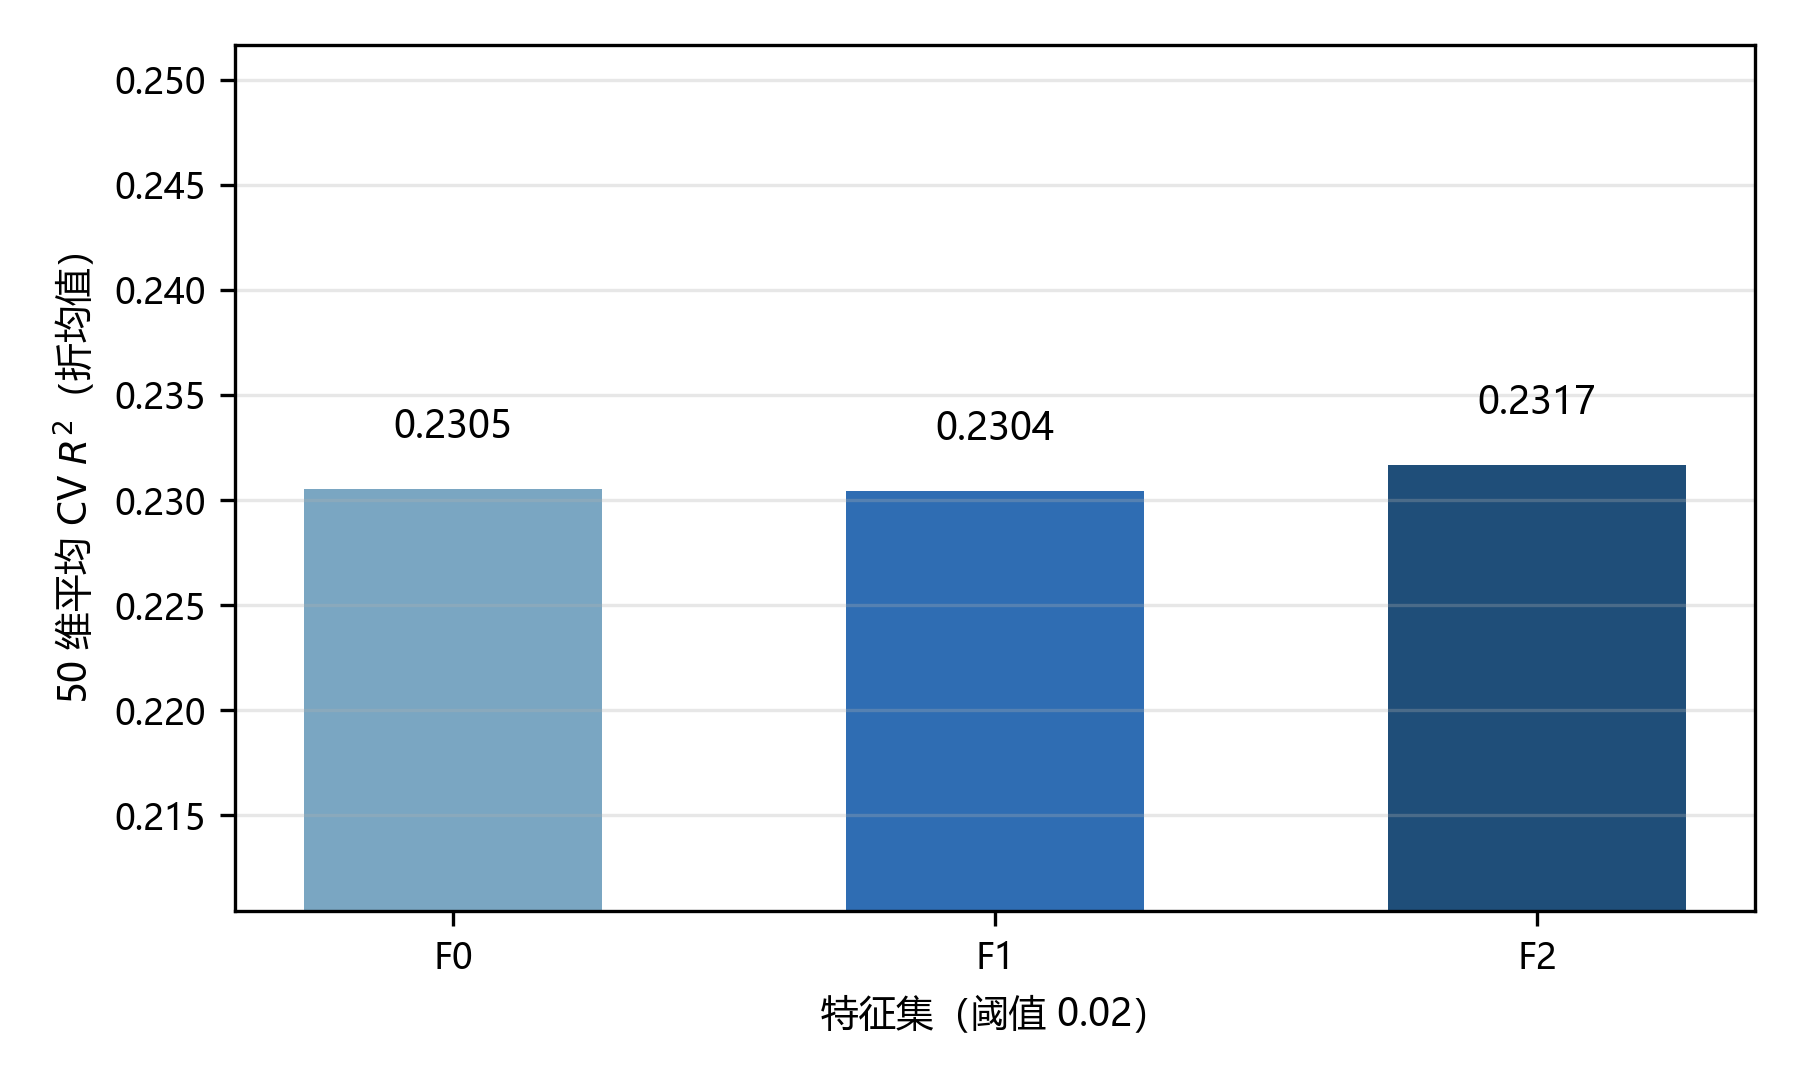
\includegraphics[width=0.64\textwidth]{图M3-02-特征集决策.png}
\caption{三套特征集在主模型下的平均交叉验证 $R^2$}
\label{fig:q1-featureset}
\end{figure}

图 \ref{fig:q1-featureset} 显示三根柱几乎等高：F2 比 F1 高 \textbf{0.0012}，F1 比 F0 低 \textbf{0.0001}。若只看“哪根柱最高”会选 F2，但预注册规则要求提升达到 \textbf{0.02} 才增加特征，因此最终采用 F0。这个结果说明，在本题的样本量下，追加 \textbf{4} 个聚合列与 \textbf{1} 个热量列没有带来可辨别的增益，保留更简的特征集反而降低了过拟合风险。

\subsubsection{逐维预测性能}

图 \ref{fig:q1-dim} 给出 \textbf{50} 个感官维度的逐维交叉验证 $R^2$，按降序排列并按香气、风味、其他三组着色。最高的是 \texttt{acetic} 的 \textbf{0.7234}，其次是 \texttt{acidity}、\texttt{alcohol}、\texttt{lactic} 和 \texttt{bitternes}；最低的是 \texttt{A\_hops\_tropical} 的 \textbf{-0.0854}，其后是 \texttt{F\_esters\_flower}、\texttt{F\_malt\_grain} 和 \texttt{A\_esters\_fruity}。前五个维度都与酸、醇、苦味等有明确化学对应的感官有关，后四个维度则更依赖品评员对细微香气的整体判断，化合物信息不足以稳定预测。

\begin{figure}[H]
\centering
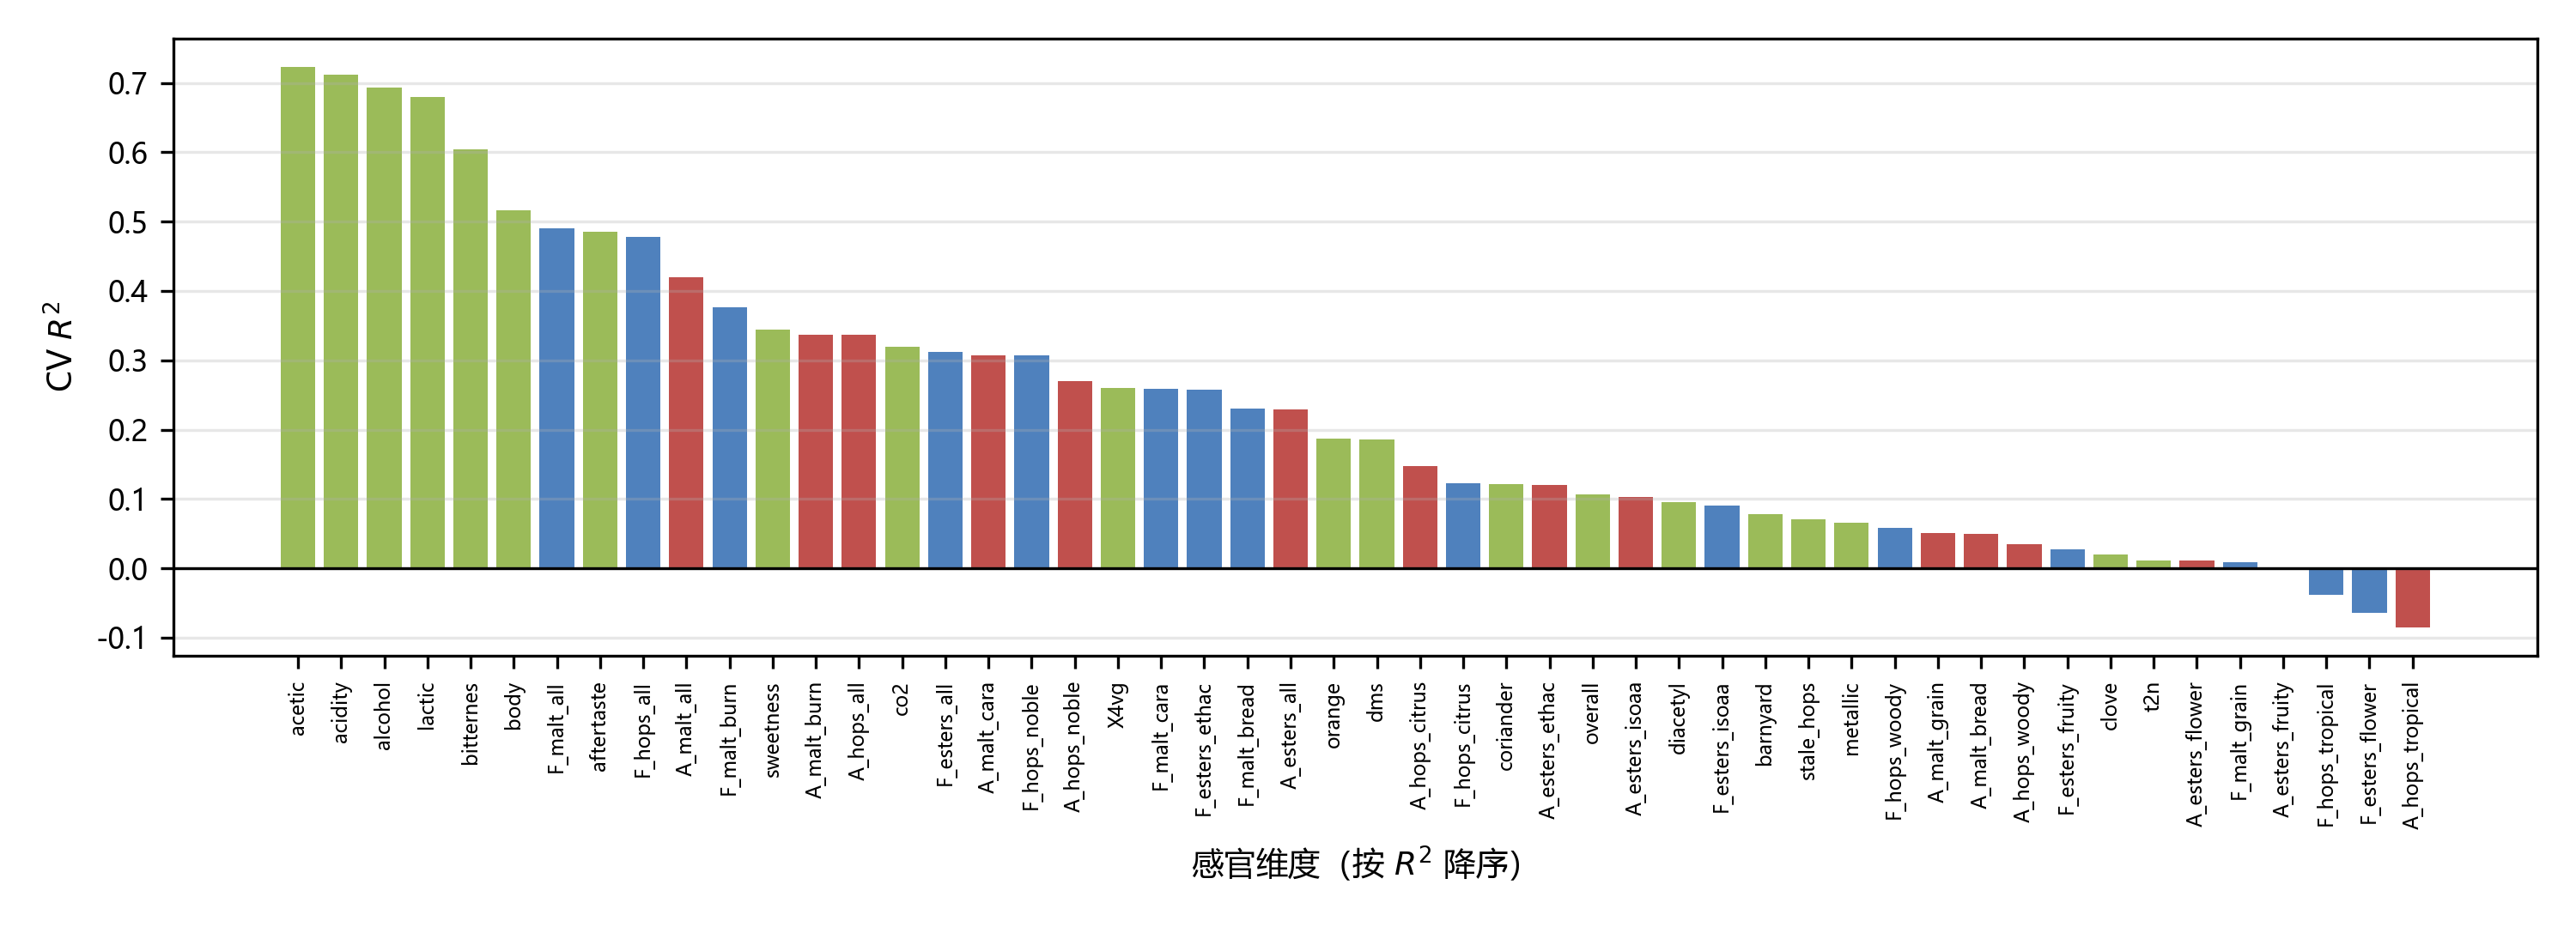
\includegraphics[width=0.96\textwidth]{图M3-03-逐维CV性能.png}
\caption{\textbf{50} 个感官维度的交叉验证 $R^2$（降序，按香气、风味、其他分组着色）}
\label{fig:q1-dim}
\end{figure}

逐维差异提示我们不要用“平均 $R^2$”掩盖结构性差异。平均 $R^2$ 为 \textbf{0.2305}，但 \textbf{50} 维中有的正值较高、有的接近零甚至为负；负值维度说明该维度的折外预测不如均值基线，本文如实保留，不删除、不单独调参。后文的 T7 信息损失与 T8 塌缩维，正是这种逐维差异在分级层面的表现。

\subsubsection{分级结果与可读口径}

把 OOF 连续预测送入 ALR 后，得到 \textbf{250}$\times$\textbf{50} 的评分表。主表的 \textbf{0} 级与 \textbf{6} 级整列为空，\textbf{5} 级只有 \textbf{23} 格，主要出现在 \texttt{bitternes}、\texttt{alcohol}、\texttt{aftertaste}、\texttt{body} 等维度；其余格子集中在 \textbf{1--4} 级。图 \ref{fig:q1-heat} 的逐维行归一化热图显示，不同维度的峰值位置不同，但两端都明显偏空。

\begin{figure}[H]
\centering
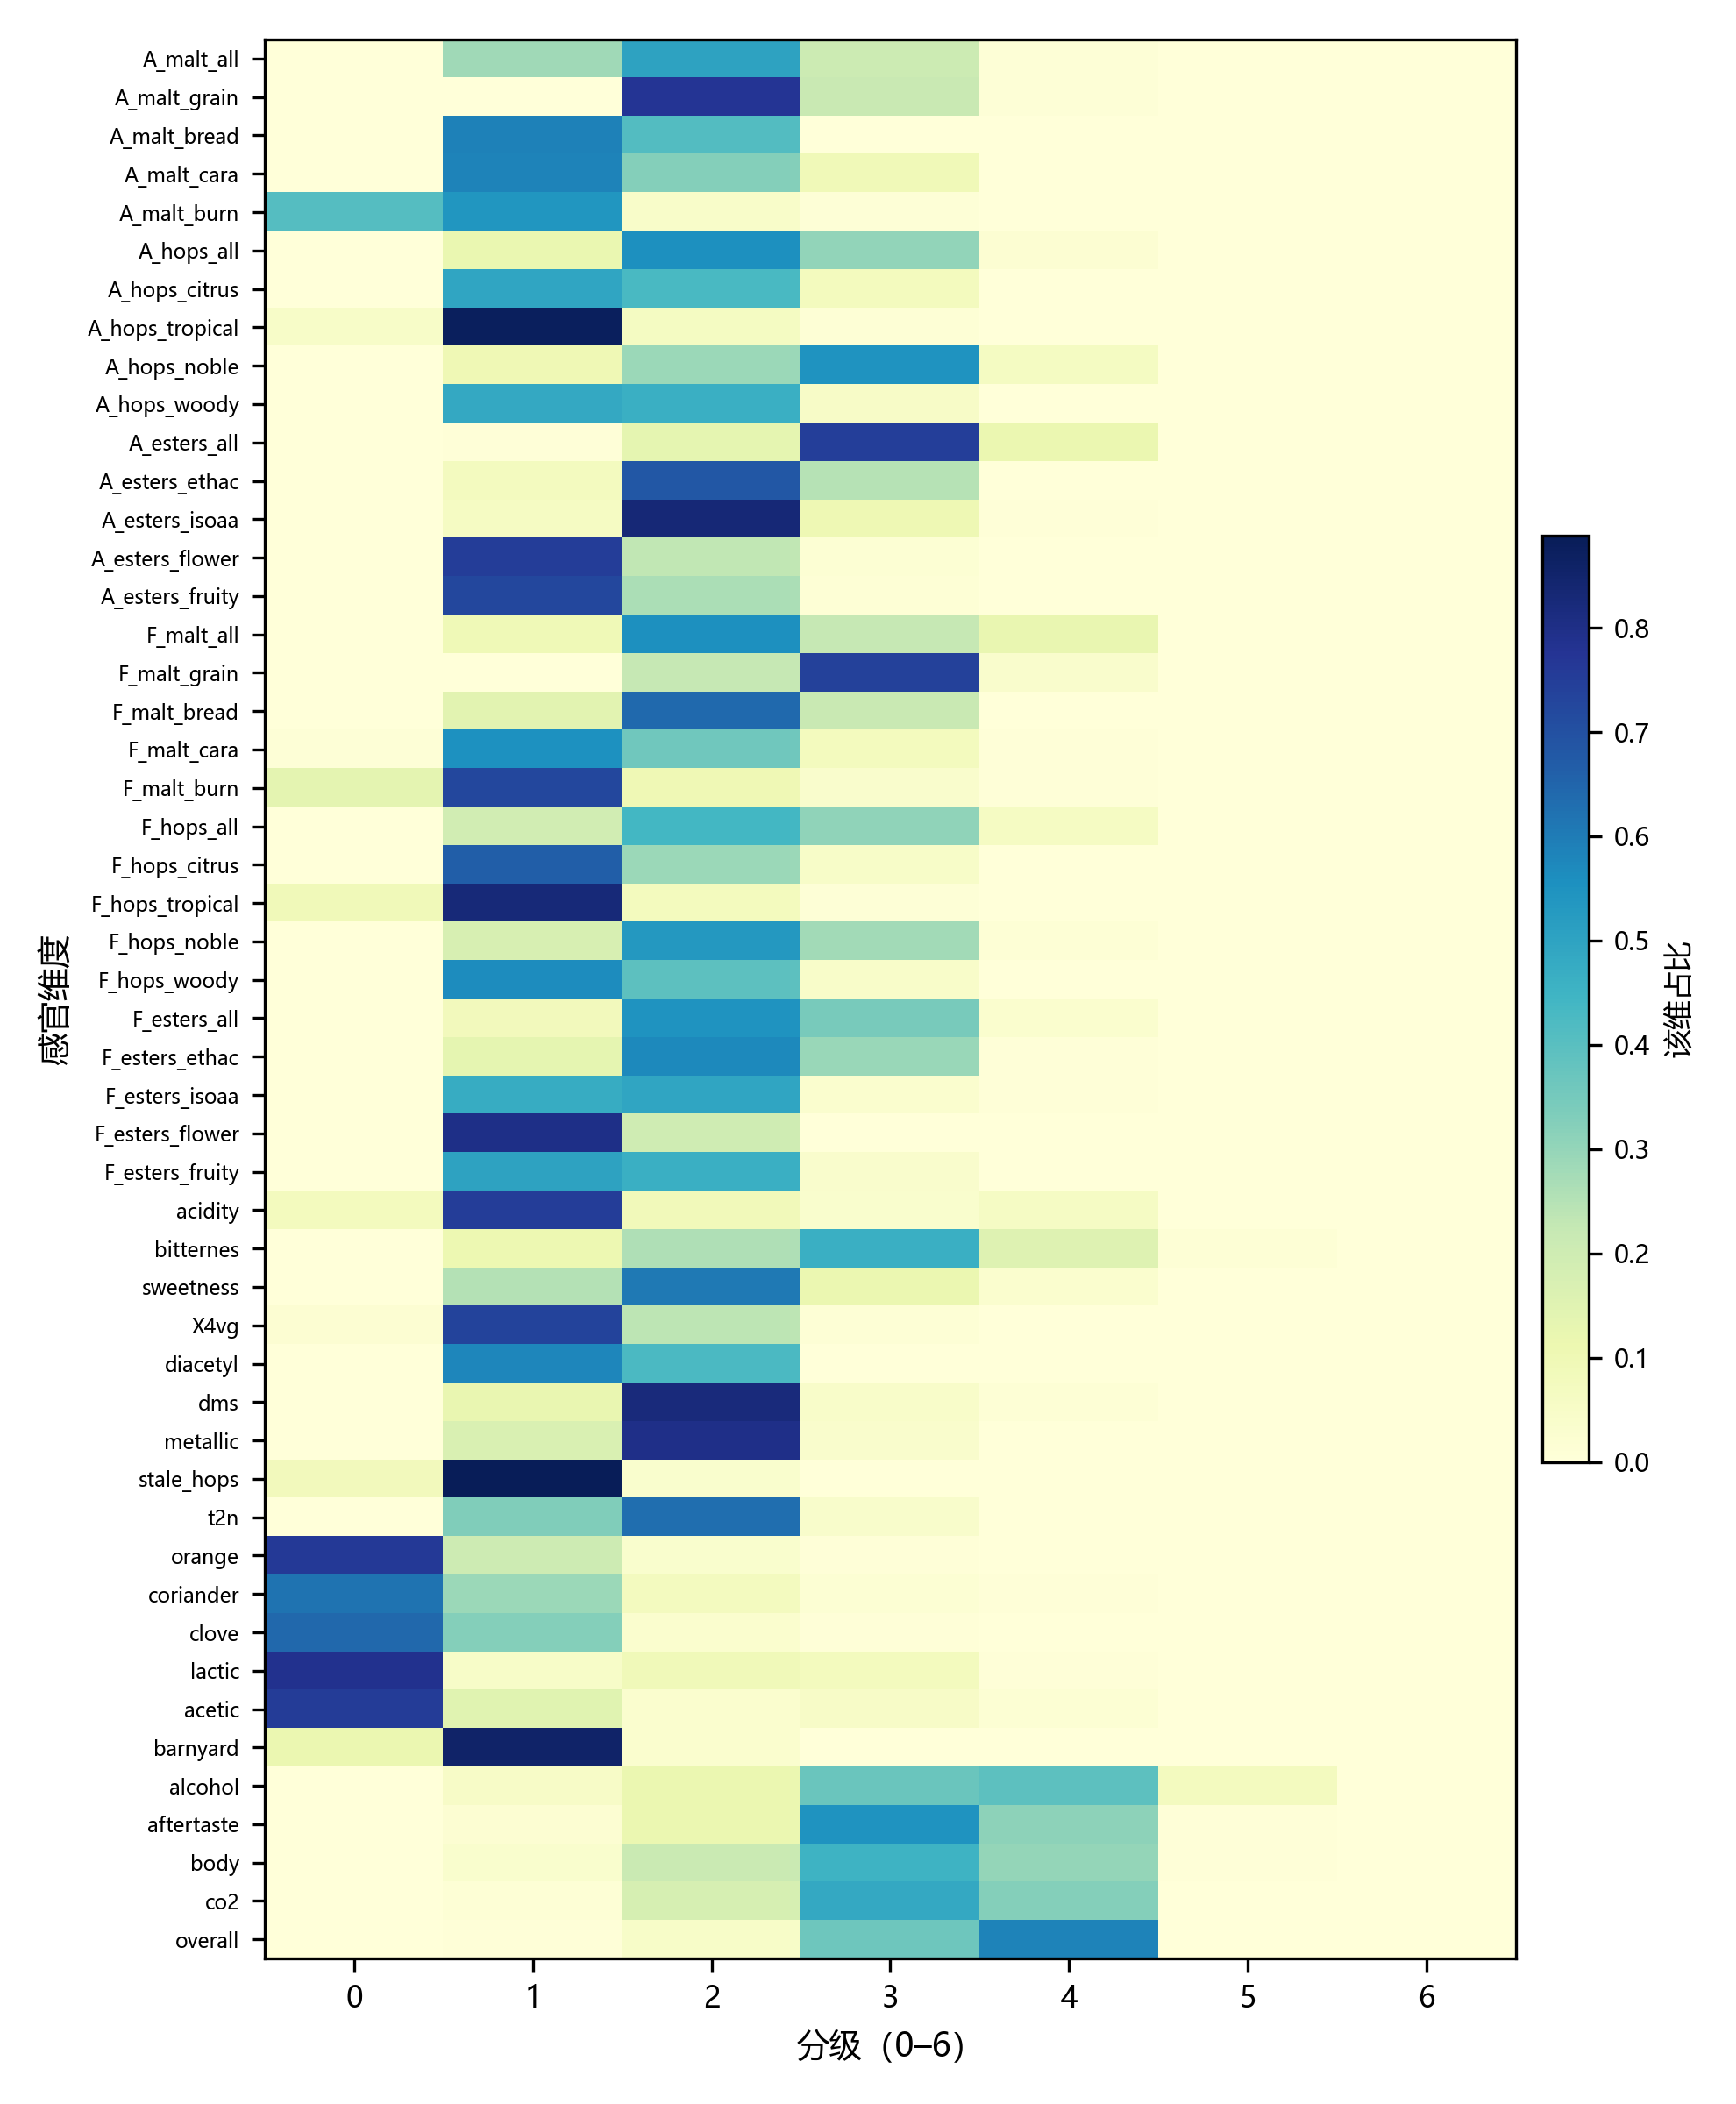
\includegraphics[width=0.56\textwidth]{图M3-04-分级分布热图.png}
\caption{主评分表 \textbf{50} 维 $\times$ \textbf{0--6} 七级的行归一化频数}
\label{fig:q1-heat}
\end{figure}

两端为空并不等于分级规则失效。T1 已证明 ALR 在规则定义域内是单调的，\textbf{50/50} 维都能在 \textbf{0--6} 的每一级取到平台；主表两端为空，是因为送入 ALR 的 OOF 预测本身值域收窄，而不是映射把两端“吃掉”了。下一小节把这个现象写成可检验的命题。

为便于按题面 \textbf{0--6} 阅读，本文另给一张可读口径辅助表。对第 $d$ 维，先把 OOF 预测做逐维单调仿射
\begin{equation}
\tilde y_d=\mu^{\mathrm{label}}_d+\left(\hat y_d-\mu^{\mathrm{pred}}_d\right)\cdot
\frac{\sigma^{\mathrm{label}}_d}{\sigma^{\mathrm{pred}}_d},
\label{eq:readable}
\end{equation}
其中 $\mu$、$\sigma$ 分别为标签与预测的均值、总体标准差；再把 $\tilde y_d$ 送入同一套 ALR 锚点。式 \eqref{eq:readable} 只改变刻度，不改变同一维度内的样本排序，因此辅助表与主表单调同序。辅助表的 \textbf{50} 维合计频数如表 \ref{tab:q1-readable} 所示，\textbf{7} 个等级全部出现，逆序对为 \textbf{0}。

\begin{table}[H]
\centering
\zihao{5}
\begin{tabularx}{\textwidth}{@{}l*{7}{r}rr@{}}
\toprule
口径 & \textbf{0} 级 & \textbf{1} 级 & \textbf{2} 级 & \textbf{3} 级 & \textbf{4} 级 & \textbf{5} 级 & \textbf{6} 级 & 合计 & 逆序对 \\
\midrule
可读口径 & \textbf{2945} & \textbf{3221} & \textbf{2634} & \textbf{2020} & \textbf{1183} & \textbf{412} & \textbf{85} & \textbf{12500} & \textbf{0} \\
\bottomrule
\end{tabularx}
\caption{可读口径辅助表的 \textbf{50} 维合计频数}
\label{tab:q1-readable}
\end{table}

表 \ref{tab:q1-readable} 的合计 \textbf{12500} 等于 \textbf{250}$\times$\textbf{50}。可读表与主表的同格率为 \textbf{55.9\%}，逐维 Spearman 在 \textbf{0.4168--0.9982} 之间；同格率不是 \textbf{100\%}，是因为式 \eqref{eq:readable} 把主表中并列的样本重新拉开，弱维的等级切点因此改变，但逆序对仍为 \textbf{0}，说明“同序”成立。缩放系数的算术平均为 \textbf{2.43}，逐维在 \textbf{1.31--3.55} 之间，量级与“预测标准差约为标签的 \textbf{0.444} 倍”一致。

\subsubsection{检验结果与刻度不可达命题}
\label{sec:q1-check}

T1--T8、E1--E3 与缺失鲁棒性的结果汇总在表 \ref{tab:q1-check}。其中 T2、T7、T8 三条不通过，本文不把它们归因于实现缺陷，而是统一写成\textbf{刻度不可达命题}：折外预测是条件均值，条件均值的方差天然小于标签方差；在近似线性、噪声与信号不相关的常见情形下，方差比 $\approx R^2$。实测逐维预测与标签的标准差之比平均为 \textbf{0.444}（范围 \textbf{0.281--0.763}），故方差比约为 $0.444^2\approx\textbf{0.197}$，与折均 $R^2$ 的 \textbf{0.2305}、OOF 全局 $R^2$ 的 \textbf{0.2565} 同阶。这个比例是 $R^2$ 小于 \textbf{1} 的直接影子，不是标定实现可以消除的偏差。

ALR 的锚点固定在标签的 \textbf{0.5\%} 与 \textbf{99.5\%} 分位数上。要得到 \textbf{6} 级，需 $s^{\ast}\ge 5.5$，即预测值至少位于锚点区间的 $5.5/6$ 处；在标签分布上，这大约对应第 \textbf{92} 百分位。一个标准差仅为标签 \textbf{0.444} 倍的预测器，要越过这一门槛的概率接近 \textbf{0}，因此主表 \textbf{6} 级为空是锚点冻结时的数学必然。\textbf{0} 级要求预测落入最低的窄带，收窄后的预测同样难以进入；\textbf{5} 级门槛在区间的 \textbf{75\%} 处，故只在少数维度出现少量格子。即 \textbf{0/6 级不可达}是口径的数学必然，而不是分级规则的实现缺陷。由同一命题可以读出三条检验的含义：

\begin{itemize}
\item \textbf{T2（保序一致）}：min Spearman 为 \textbf{0.6575}。ALR 规则本身单调（T1 的 \textbf{50/50} 维通过），T2 偏低来自标签在 \textbf{0} 级的大量并列，例如 \texttt{acetic} 有 \textbf{82.8\%} 的样本落在 \textbf{0} 级；并列越多，Spearman 的惩罚越重。
\item \textbf{T7（信息损失）}：min Spearman 为 \textbf{0.5470}。分级把连续预测压成少数等级，等级越少、并列越多，分级与连续预测的秩相关越低；这是离散化本身的信息损失，不是预测器换了目标。
\item \textbf{T8（塌缩维）}：实际使用等级数不超过 \textbf{3} 的维度有 \textbf{19} 个，其中 \textbf{3} 个维度只用了 \textbf{2} 级。原方案要求塌缩维不超过 \textbf{5}，该阈值与本方案冻结的标签锚点不相容；按同一锚点，收窄预测必然集中在中间等级。
\end{itemize}

\begin{table}[H]
\centering
\zihao{-5}
\begin{tabularx}{\textwidth}{@{}p{0.08\textwidth}p{0.20\textwidth}p{0.18\textwidth}p{0.16\textwidth}X@{}}
\toprule
编号 & 指标 & 实测 & 判据 & 结论与解释 \\
\midrule
T1 & 单调性（\textbf{50} 维） & \textbf{50/50} 通过 & 非降且 \textbf{0--6} 平台齐全 & 通过 \\
T2 & 保序一致 min Spearman & \textbf{0.6575} & $\ge 0.99$ & 不通过；刻度不可达（标签并列） \\
T3 & 参考分级等级数 & \textbf{45} 维 \textbf{7} 级、\textbf{5} 维 \textbf{6} 级 & min $\ge 5$ & 通过 \\
T4 & 边界确定性（\textbf{50} 维） & \textbf{50/50} 通过 & 六类输入一致 & 通过 \\
T5 & 往返复原 & \textbf{12500/12500} & $=1.0$ & 通过 \\
T6 & 锚点敏感性均值 & \textbf{0.8308}；P1/P99 为 \textbf{0.8890} & 只报告 & 记录 \\
T7 & 信息损失 min Spearman & \textbf{0.5470} & $\ge 0.95$ & 不通过；刻度不可达（离散损失） \\
T8 & 塌缩维 / 仅 \textbf{2} 级维 & \textbf{19} / \textbf{3} & 塌缩维 $\le 5$ & 不通过；刻度不可达（阈值冲突） \\
E1 & 有效格 / 化合物 & \textbf{949/2200}；\textbf{42} 个 & 平均绝对差 $\le 0.25$ & 通过；\textbf{0.1201}，方向一致率 \textbf{0.9968} \\
E2 & 感官协同结构 & \textbf{1225} 对；\textbf{0.1719} & 平均绝对差 $\le 0.20$ & 通过；方向一致率 \textbf{0.8098} \\
E3 & 独立方向证据 & \textbf{39} 映射 / \textbf{34} 有效 & $N_{\mathrm{eff}}\ge 20$ 且 $R_3\ge 0.60$ & 通过；$R_3=\textbf{0.9706}$ \\
鲁棒性 & 缺失 \textbf{20\%} & 折均 \textbf{0.2121}；一致率 \textbf{0.8882} & 记录 & 下降可控 \\
\bottomrule
\end{tabularx}
\caption{问题一的检验、独立证据与缺失鲁棒性汇总}
\label{tab:q1-check}
\end{table}

表 \ref{tab:q1-check} 的 T2、T7、T8 三行都应在“刻度不可达命题”下阅读：T2 是标签并列造成的秩相关下降，T7 是离散化造成的信息损失，T8 是阈值与冻结锚点不相容。三者都不是“换一个模型就能变好”的执行问题；若强行拉伸预测去填满 \textbf{0} 级与 \textbf{6} 级，反而会破坏锚点语义，让评分表与连续预测不再同序。本文的选择是保留主表、如实登记，并用可读口径辅助表解决“看起来没有 \textbf{6} 级”的阅读问题。

\subsubsection{独立证据与缺失鲁棒性}

缺失鲁棒性通过人工遮蔽测试折的 \textbf{5\%}、\textbf{10\%}、\textbf{20\%} 个格子来检验。折均 $R^2$ 从 \textbf{0.2305} 降到 \textbf{0.2266}、\textbf{0.2256}、\textbf{0.2121}，分级一致率从 \textbf{1.0000} 降到 \textbf{0.9658}、\textbf{0.9348}、\textbf{0.8882}。图 \ref{fig:q1-mask} 的左图是 $R^2$ 的下降曲线，右图是一致率曲线；两条曲线在 \textbf{10\%} 以内都比较平，到 \textbf{20\%} 才明显下弯，说明模型对偶发缺失有缓冲，但不适合在缺失率很高时直接使用。

\begin{figure}[H]
\centering
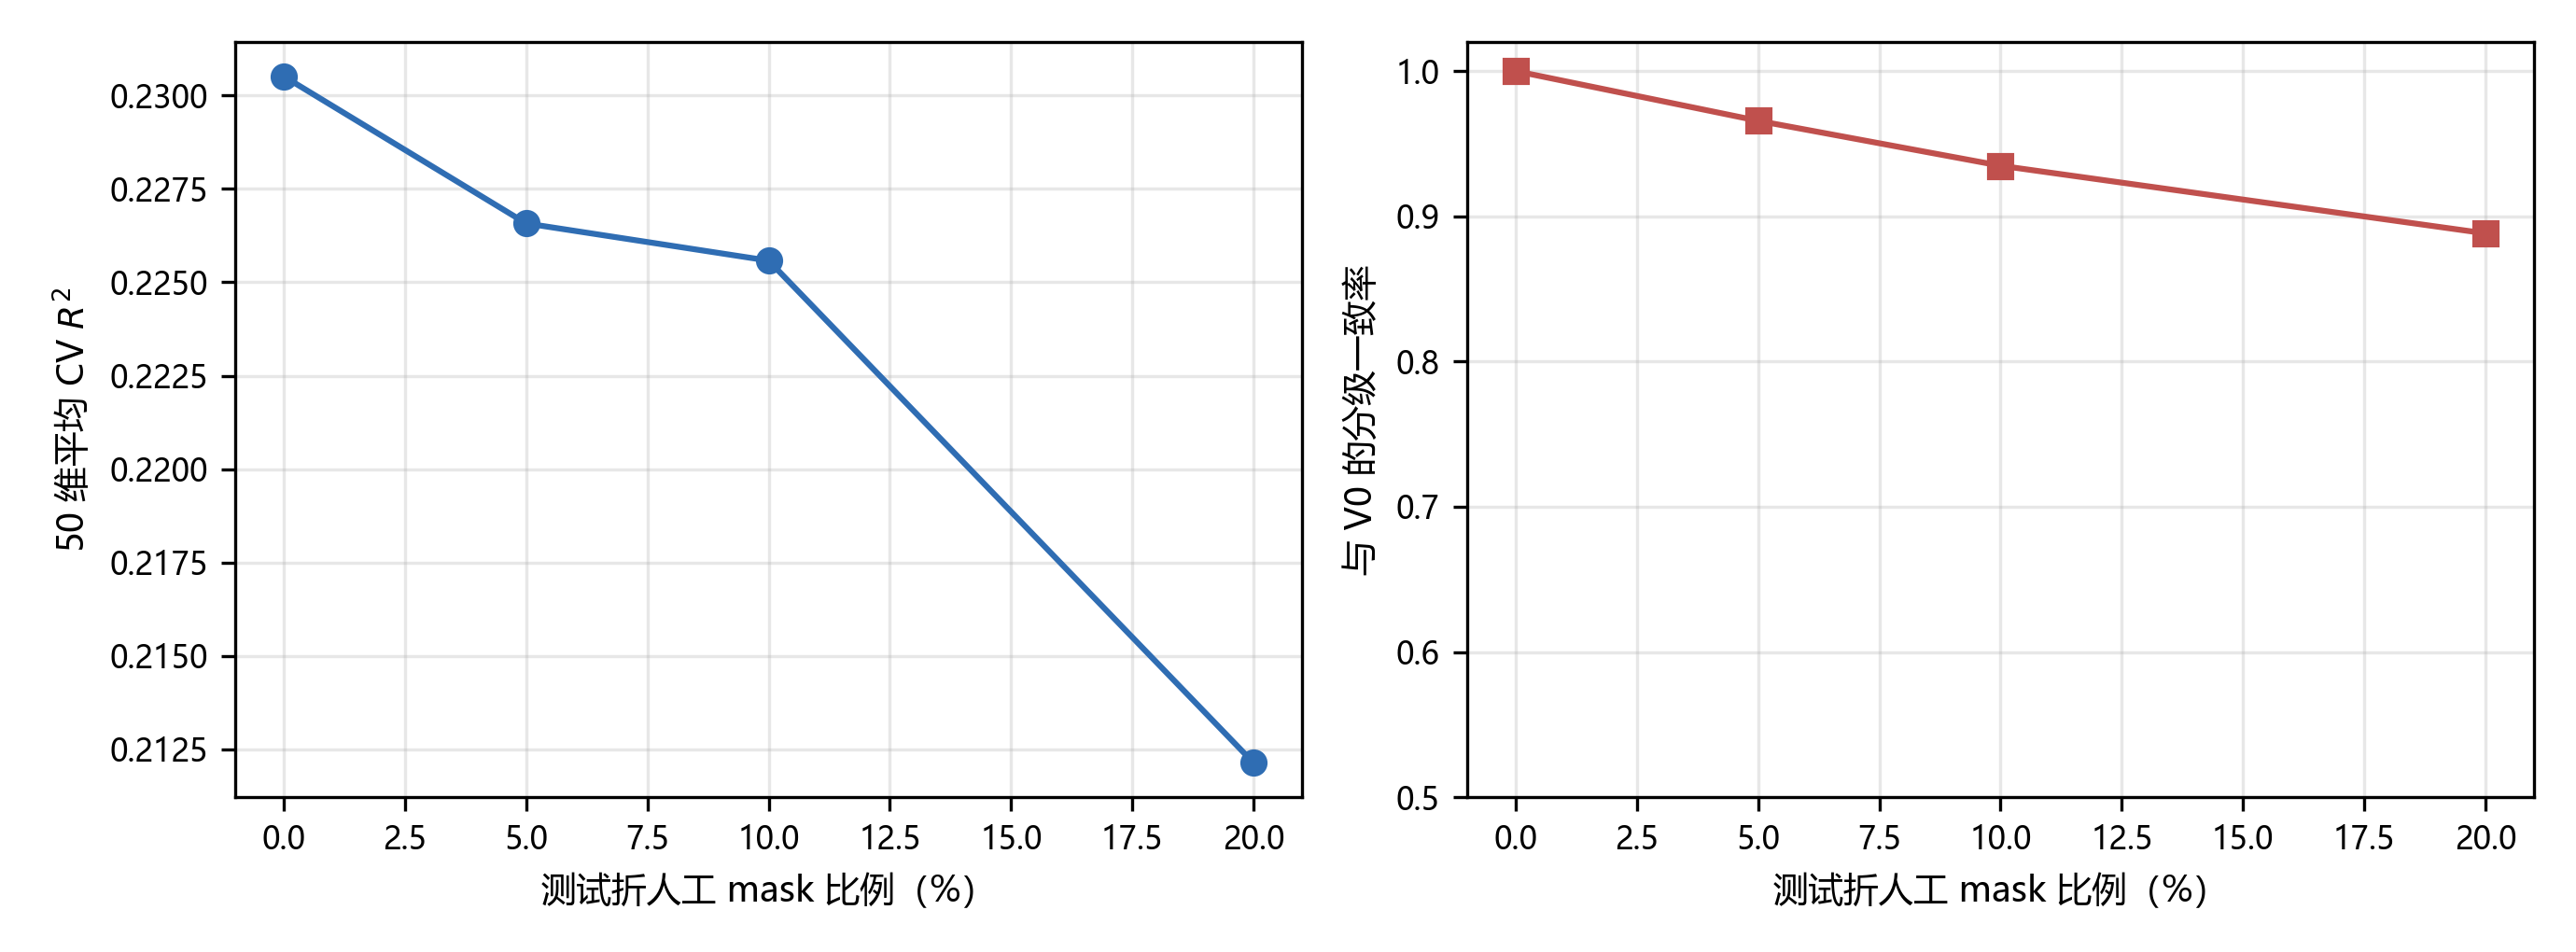
\includegraphics[width=0.92\textwidth]{图M3-05-缺失鲁棒性.png}
\caption{人工缺失比例对折均 $R^2$ 与分级一致率的影响}
\label{fig:q1-mask}
\end{figure}

E1 用 \texttt{6.csv} 的参考相关核对 OOF 预测重算的相关结构。\texttt{6.csv} 有 \textbf{44} 个指标，其中 \textbf{42} 个能映射到 \texttt{1.csv}；在 \textbf{2200} 个格子里有 \textbf{949} 个有效格，平均绝对差为 \textbf{0.1201}，方向一致率为 \textbf{0.9968}。图 \ref{fig:q1-e1} 的散点沿对角线分布，说明预测重算的相关方向与题方参考相关基本一致；偏离主要出现在参考相关接近 \textbf{0} 的格子，此时方向本身不稳定。

\begin{figure}[H]
\centering
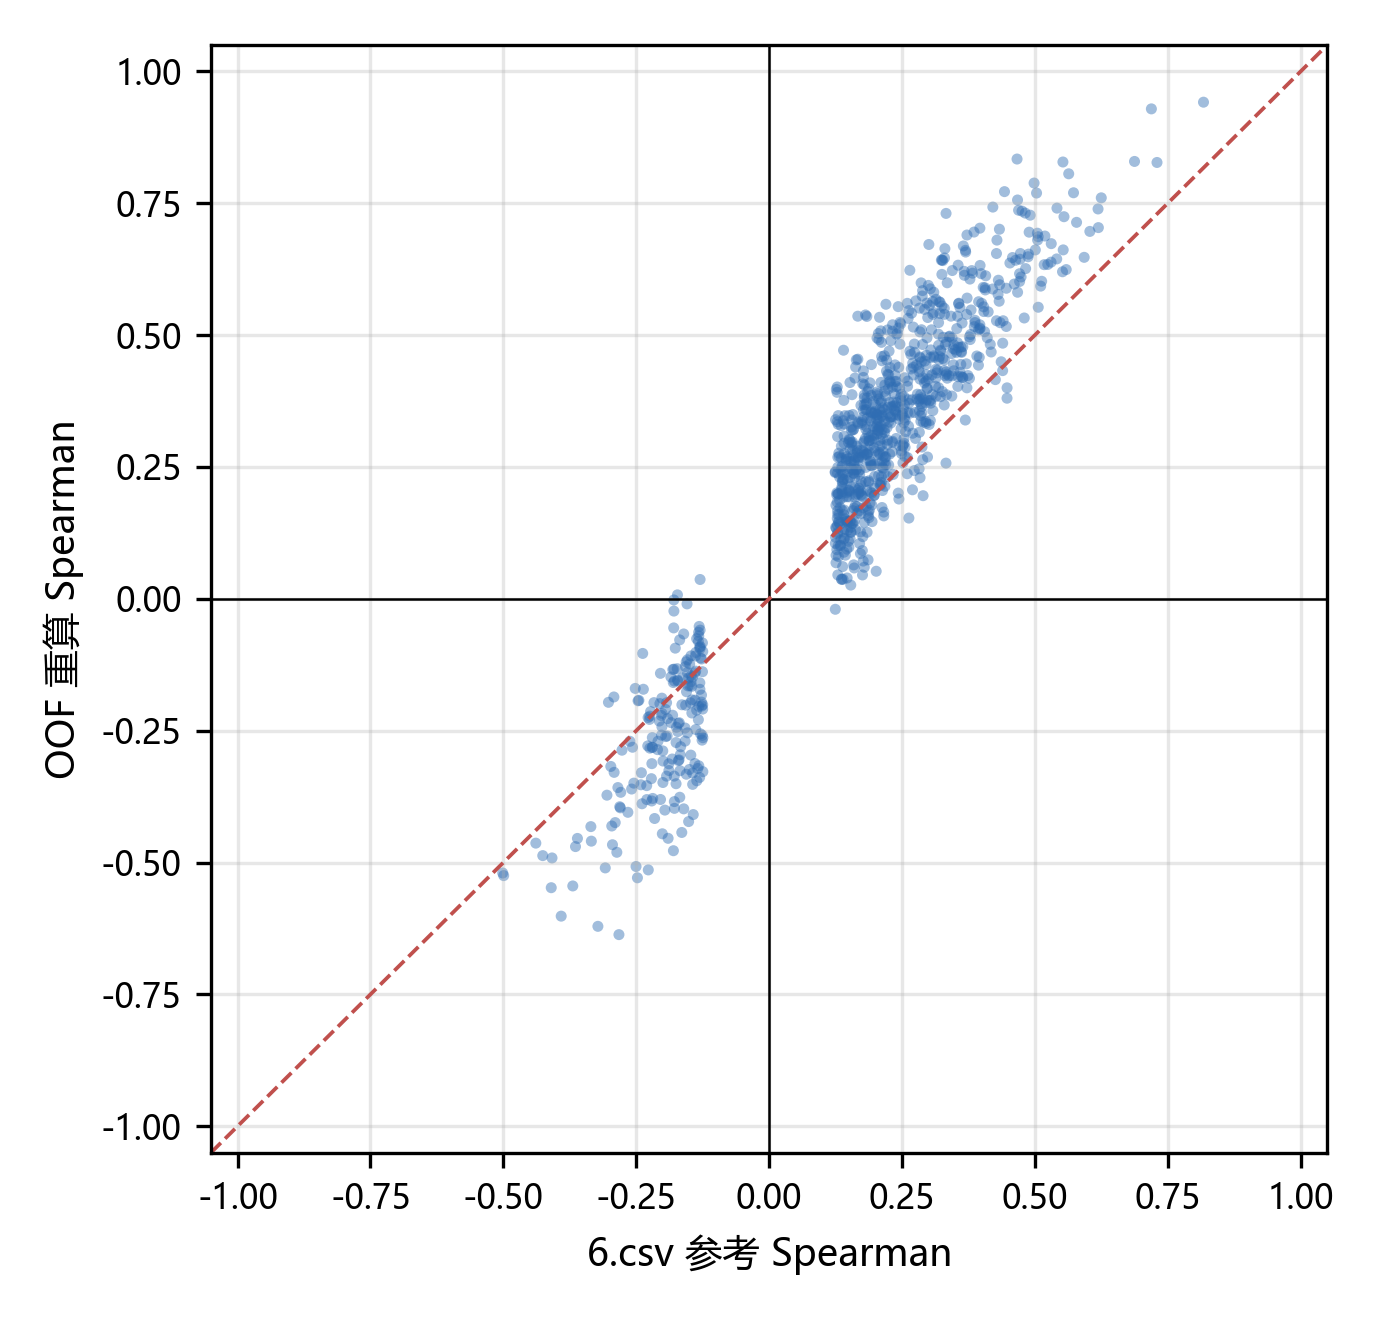
\includegraphics[width=0.46\textwidth]{图M3-06-E1方向散点.png}
\caption{题方 \texttt{6.csv} 参考 Spearman 与 OOF 重算 Spearman 的逐格对照}
\label{fig:q1-e1}
\end{figure}

E2 用 \texttt{5.csv} 的 \textbf{50}$\times$\textbf{50} 感官相关阵核对预测矩阵的列间结构，\textbf{1225} 对的平均绝对差为 \textbf{0.1719}，方向一致率为 \textbf{0.8098}，低于 E1 但仍在判据内；这说明模型不仅拟合了单维均值，也保留了一部分感官维度之间的协同结构。E3 把 \texttt{7.csv} 的 \textbf{186} 个属性桥接到感官维度，得到 \textbf{39} 个可映射属性、\textbf{34} 个有效映射，方向一致率 $R_3$ 为 \textbf{0.9706}，说明预测方向与独立属性证据一致。

\subsubsection{小结}

问题一的主线可以概括为“随机森林拟合连续评分、ALR 转成等级、刻度不可达命题解释两端为空”。主模型在 OOF 全局口径下为 \textbf{0.2565}，折均口径下为 \textbf{0.2305}，都高于同口径基线；逐维差异、T2/T7/T8 的偏离、E1--E3 的独立证据与缺失鲁棒性共同说明：模型在平均意义上有效，在弱维和两端等级上存在结构性限制。可读口径辅助表在不改变主表排序的前提下补足 \textbf{7} 级覆盖，为后续展示与使用提供了更友好的界面。
